\section{Out-of-equilibrium dynamics arising from a dissipation hole}

\begin{figure}[!b]
    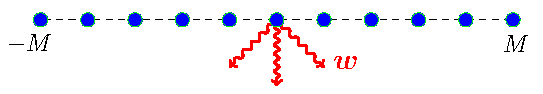
\includegraphics[width=1.0\columnwidth]{imm/sketch.eps}
    \caption{Sketch of a fermionic chain of size $L=2M+1$ subject to a
      localized particle loss at the central site, with strength
      controlled by the dissipation parameter $w$.  }
    \label{fig:sketch}
  \end{figure}
  
  
  As paradigmatic models we consider one-dimensional lattice models of
  non-interacting spinless fermionic gases, within hard-wall and
  harmonic traps, subject to dissipative perturbations that give rise to
  a particle loss localized at one of the sites of the lattice, such as
  the set up sketched in Fig.~\ref{fig:sketch}.  We model the
  dissipative particle-decay mechanism by Lindblad master equations
  governing the time evolution of the density
  matrix~\cite{Lindblad-76,GKS-76,BP-openquantumsystembook,RH-book,dr2021self}.  To
  investigate the effects of the localized particle-loss dissipation, we
  study the quantum dynamics arising from protocols starting from the
  ground state of the fermionic gas, then evolving under the effect of
  the particle-loss dissipation, for example localized at the center of
  the system.  This is analyzed in the large-$\ell$ limit for two
  different initial conditions: fixed number $N_0$ of initial particles
  and fixed ratio $N_0/\ell$, which corresponds to the {\em
    thermodynamic} limit of the initial fermionic gases at equilibrium,
  in both hard walls and harmonic traps.  The quantum evolution of the
  particle number and space-dependent density turns out to develop
  various dynamic scaling regimes, and nontrivial large-time behaviors
  when the dissipative mechanism acts at the center of the system.
  
  Some issues concerning the behavior of fermionic gases in the presence
  of localized dissipative interactions have been already discussed in
  Refs.~\cite{FCKD-19,LHFHCE-19,KMS-19,WSDK-20,FMKCD-20}, mainly
  for homogeneous systems neglecting boundary effects. Here we extend
  these studies by analyzing the interplay between time, size of the
  system, and number $N_0$ of initial particles. We analyze the various
  large-time and intermediate dynamic regimes, in both homogeneous
  particle systems within hard walls and inhomogeneous particle systems
  in harmonic traps. Substantially different and peculiar behaviors are
  observed in fermionic gases confined by hard walls and harmonic traps.
  
  
  The understanding of the interplay between the time dependence and the
  finite size of the system is essential to interpret results in various
  experimental contexts. For example this issue is fundamental for
  small-size quantum simulators operating on a limited amount of quantum
  objects, in the presence of controlled dissipation. We also mention
  experiments with cold atoms within a trap of finite size, when the
  many-body correlations become eventually sensitive to the trapping
  potential (local density approximations generally fail to describe
  quantum correlations, in particular when they are
  critical~\cite{CTV-13} and/or out-of-equilibrium~\cite{rossini2021coherent}).
  
  
  \subsection{Free lattice fermions  with localized dissipative defects}
  \label{modeldiss}
  
  \subsubsection{The Hamiltonian}
  \label{model}
  
  We consider one-dimensional $N$-particle Fermi gases defined on a
  chain with $L=2M+1$ sites, by the Hamiltonian
  \begin{equation}
    \hat H =
    - \kappa \sum _{x=-M}^{M-1} 
    (\hat c_{x}^\dagger \hat c_{x+1} +  \hat c_{x+1}^\dagger \hat c_{x})\,,
    \label{Hfree}
  \end{equation}
  where $\hat c_x$ is a fermion one-particle operator, and $\hat n_x =
  \hat c_x^\dagger c_x$ is the particle density operator.  We consider
  hard-wall (open) boundary conditions.  The site $x=0$ is the central
  site of the chain.  In the following we set $\hslash=1$ and $\kappa=1$
  without loss of generality.
  
  We also consider fermionic systems where the particles are trapped by
  an external potential, which can be taken into account by adding a
  corresponding term to the Hamiltonian (\ref{Hfree}), such as
  \begin{eqnarray}
    \hat H_t =
    - \sum _x 
    (\hat c_{x}^\dagger \hat c_{x+1} +  \hat c_{x+1}^\dagger \hat c_{x})
  +  \sum_x V(r) \, \hat n_x\,,\label{htrap}
    \end{eqnarray}
  where 
  \begin{eqnarray}
  \hat n_x =
  \hat c_x^\dagger c_x\,,\quad  V(r)= (r/L_t)^p\,, \quad r\equiv |x|\,,
     \label{potential}
  \end{eqnarray}
  $p$ is a positive number, $r$ is the distance from the center $x=0$ of
  the trap, and $L_t$ plays the role of trap size.~\footnote{$L_t$ plays
  the role of trap size~\cite{BDZ-08,RM-04,CV-10-2}, so that the {\em
    thermodynamic} limit is obtained in the large trap-size limit,
  $L_t\to \infty$, keeping the ratio between the particle number $N$ and
  the trap size $L_t$ constant, which can be equivalently obtained by
  adding a chemical-potential term in the Hamiltonian, such as the one
  reported in Eq.~(\ref{chemicalpot}).}  The trapping potential is
  effectively harmonic in most cold-atom experiments~\cite{BDZ-08},
  i.e., $p=2$.  In the limit $p\to\infty$ we recover the model
  (\ref{Hfree}) with hard-wall boundary conditions and $M=\lfloor L_t
  \rfloor$.  The size of systems described by the Hamiltonian $\hat H_t$
  with finite $p$ is supposed to be infinite. However for practical
  purposes it is sufficient to consider models within hard walls with $L
  \gg L_t$. Indeed the large-size convergence is generally fast for
  sufficiently large values of $p$, including $p=2$, due to the fact
  that the average particle density $\langle \hat{n}_x \rangle$ vanishes
  rapidly for $|x|\gg L_t$. The main features of the behavior of fermionic
  gases trapped by a inhomogeneous external power-law potentials have
  been much investigated, see e.g.
  Refs.~\cite{ACV-14,Nigro-17,CV-10,CV-10-2,Pollet-12}.
  
  In systems within both hard-wall and inhomogeneous traps, the particle
  number operator
  \begin{equation}
    \hat{N} = \sum_x \hat n_{x}\,
  \label{partnum}
    \end{equation}
  commutes with both Hamiltonians (\ref{Hfree}) and
  (\ref{htrap}). Therefore the particle number is conserved in both
  cases.  In the following we consider ground states for a number $N_0$
  of particles as starting point of dynamic protocols involving
  dissipative mechanisms.
  
  
  
  \subsubsection{Localized particle-decay dissipation}
  \label{locdiss}
  
  We model the dissipative mechanisms within the Lindblad
  framework~\cite{Lindblad-76,GKS-76}, where the evolution of the matrix
  density $\rho(t)$ of the system is described by he
  equation~\cite{BP-openquantumsystembook,RH-book}
  \begin{eqnarray}
  &&  {\partial\rho\over \partial t} = {\cal L}[\rho]=
    - i \, [ \hat H,\rho]
    + {\mathbb D}[\rho]\,.
    \label{EQLindblad}
  \end{eqnarray}
  We recall that the conditions leading to the Lindblad framework are
  typically satisfied in quantum optical
  implementations~\cite{BDS-2015-KeldyshOptical,dr2021self}.  The form of the operator
  ${\mathbb D}[\rho]$ depends on the nature of the dissipation arising
  from the interaction with the bath.  We consider a localized
  particle-decay dissipation acting at the site $z$, modeled by the
  Lindblad operator~\cite{HC-13, KMSFR-17, N-2019-uniquenesslindblad, NRV-2019-competingdissipativeandcoherent, WSDK-20,
    FMKCD-20, dr2021self,rossini2021coherent}
  \begin{eqnarray}
  \mathbb{D}[\rho] = w\,\biggr[
      \hat c_{z}\,\rho\,\hat c_{z}^\dagger - {1\over 2}\left( \rho\,
      \hat c_z^\dagger \hat c_{z} + \hat c_z^\dagger \hat c_{z} \rho \right)
      \biggr] \,, 
  \label{Lindop}
  \end{eqnarray}
  where $w$ is a parameter controlling the strength of the particle-loss
  dissipation.
  Note that reflection symmetry with respect to
    the center of the confined particle system is only preserved when
    the particle-loss dissipation is localized at the center. As we
    shall see, this will lead to peculiar behaviors with respect to the
    case of particle-loss dissipation localized at generic sites.
  
  
  
  The approach to the asymptotic stationary states are generally
  controlled by the Liouvillian gap $\Delta_{\cal L}$ associated with
  the generator ${\cal L}$ entering the Lindblad equation
  (\ref{EQLindblad})~\cite{BP-openquantumsystembook,RH-book,Z-2015-relaxtimes,MBBC-18,KS-2020-boundarydephasing}.
  The asymptotic stationary state is provided by the eigenstate of
  ${\cal L}$ with vanishing eigenvalue, $\Lambda_0=0$, while all other
  eigenstates have eigenvalues $\Lambda_i$ with negative real part,
  i.e. ${\rm Re}\,\Lambda_i<0$ for any $i>0$.
  
  
  \subsubsection{Dynamic protocol}
  \label{dynprot}
  
  To study fermionic gases under the effects of a localized
  particle-loss mechanism, we consider the following dynamic protocol,
  for systems within both hard-wall and harmonic traps, respectively of
  size $L=2M+1$ and $L_t$.
  
  \begin{itemize}
  
  \item[$\bullet$] The protocol starts at time $t=0$ from the ground
    state of the Hamiltonian (\ref{Hfree}) or (\ref{htrap}) with a
    number $N_0$ of particles. We recall that the ground state of $N_0$
    noninteracting fermionic particles is obtained by filling the lowest
    $N_0$ one-particle energy levels.
  
  \item[$\bullet$] The time evolution for $t>0$ is driven by the 
    Lindblad equation (\ref{EQLindblad}) for the density matrix
    $\rho(t)$, with particle-decay dissipation localized at a site $z$
    and controlled by the parameter $w$.
  
  \item[$\bullet$]
  The particle density and total particle number,  
  \begin{eqnarray}
  n_x(t) = {\rm Tr}[ \rho(t) \hat n_x ] \,,\qquad
  N(t) = {\rm Tr}\Bigr[ \rho(t) \hat N \Bigr] \,,
  \label{nxntdef}
  \end{eqnarray}
  are monitored during the out-of-equilibrium evolution for $t>0$, up to
  their large-time behaviors.
  
  \end{itemize}
  
  To compute the particle density $n_x(t)$ and particle number $N(t)$,
  we proceed as follows.  We introduce the correlation functions
  \begin{eqnarray}
    {\mathscr C}_{x,y}(t)= {\rm Tr}\Bigr[ \rho(t) \, \hat c_x^\dagger
      \hat c_y \Bigr] \,.
  \label{defct}
  \end{eqnarray}
  For homogeneous systems described by the Hamiltonian (\ref{Hfree}),
  the Lindblad equation (\ref{EQLindblad}) 
  implies
  \begin{eqnarray}
    {d\mathscr{C}_{x,y}\over dt} &=& i\,( \mathscr{C}_{x,y+1} -
     \mathscr{C}_{x-1,y} + \mathscr{C}_{x,y-1} - \mathscr{C}_{x+1,y} )
        \nonumber\\
      &&- \frac{w}{2} \ ( \delta _{z,y} + 
     \delta _{x, z} ) \, \mathscr{C}_{x,y} \,,
     \label{eqscxy}
  \end{eqnarray}
  where $\delta_{x,x}=1$ and $\delta_{x,y}=0$ for $x\neq y$.  Since we
  consider open (hard-wall) boundary conditions, ${\mathscr
    C}_{xy}(t)=0$ when the coordinates $x$ or $y$ refer to sites outside
  the space interval $[-M,M]$.  An analogous equation can be derived in
  the presence of an inhomogeneous external trapping potential,
  cf. Eq.~(\ref{htrap}).  We obtain
  \begin{eqnarray}
    &&  
    {d\mathscr{C}_{x,y}\over dt} = i\,( \mathscr{C}_{x,y+1} -
     \mathscr{C}_{x-1,y} + \mathscr{C}_{x,y-1} - \mathscr{C}_{x+1,y} )
     \nonumber\\
  &&\;\; + i {|x|^p - |y|^p\over L_t^p} \mathscr{C}_{x,y} 
  - \frac{w}{2} \ ( \delta _{z,y} + 
     \delta _{x, z} ) \, \mathscr{C}_{x,y} \,.
     \label{eqscxytrap}
  \end{eqnarray}
  Then, after numerically solving the above equations, we use the
  relations
  \begin{equation}
  n_x(t)=\mathscr{C}_{x,x}(t) \,,\qquad   N(t) = \sum _x n_x\,.
  \label{ntcxy}
  \end{equation}
  
  One can easily check that for both hard-wall and harmonic traps the
  derivative of the particle number is proportional to the average
  particle density $n_z$ at the site $z$ where the particle-decay
  dissipation is localized, i.e.
  \begin{equation}
    {d N(t)\over dt} = - w \, n_z(t) < 0\,.
  \label{ntnz}
  \end{equation}
  Therefore the particle number decays monotonically, since $n_z(t)\ge
  0$, and the particle loss stops if $n_z(t)= 0$ asymptotically.
  
  One may also consider the energy of the system, defined as
  \begin{eqnarray}
  E(t) = {\rm Tr}[\rho(t) \hat H] \,,
  \label{enedef}
  \end{eqnarray}
  for which the Lindblad equation implies
  \begin{eqnarray}
    {d E(t)\over dt} = {\rm Tr}\left[{d\rho(t)\over dt} \hat H\right]= w
    {\rm Tr}[{\mathbb D}[\rho] \,\hat H]\,.
    \label{detg}
  \end{eqnarray}
  For systems with particle-loss dissipation localized at the central
  site $x=0$, we obtain
  \begin{eqnarray}
    {d E(t)\over dt} =
    w \, {\rm Re}\,({\mathscr C}_{0,1}+{\mathscr C}_{-1,0}) =
    2 w \, {\rm Re}\,{\mathscr C}_{0,1}\,,
    \label{derene}
  \end{eqnarray}
  which holds for systems within hard walls and also inhomogeneous
  traps.
  
  \subsection{Fermi gases within hard walls}
  \label{hwbc}
  
  In this section we consider homogeneous Fermi chains, cf.
  Eq.~(\ref{Hfree}), and discuss the dynamic evolution under the
  particle-loss dissipation described by the Lindblad equation
  (\ref{EQLindblad}), in particular Eq.~(\ref{eqscxy}). For this
  purpose, we numerically solve the differential equation (\ref{eqscxy})
  using the fourth-order Runge-Kutta method (with an accuracy of
  approximately $10^{-8}$ on the evolution of the particle number).
  
  We study the interplay between the time dependence, the number $N_0$
  of initial particles and the size $L=2M+1$ of the lattice.  For this
  purpose we consider two different situations: (i) the number $N_0$ of
  particles is kept fixed while increasing $M$; (ii) the number of
  particles is increases as $N_0\sim M$, so that the ratio $N_0/M$
  fixed, while increasing $M$. Note that the latter condition can be
  equivalently realized in the large-size limit by adding a chemical
  potential to the Hamiltonian (\ref{Hfree}), i.e.
  \begin{equation}
  \hat H_\mu = -(\mu+2) \sum _x \hat n_x \,.
  \label{chemicalpot}
  \end{equation}
  The value $\mu=\mu_{\rm vs}=-2$ corresponds to the vacuum-superfluid
  transition point~\cite{S99,ACV-14}, separating the phase
  where the lowest Hamiltonian eigenstate has $N=0$ particles from the
  one for $\mu>-2$ where the ground-state has $N\sim L$ fermions.
  
  In the following we first analyze the asymptotic large-time regime.
  Then we show that the time dependence of the particle number develops
  various asymptotic and intermediate regimes, which may differ in the
  cases we keep $N_0$ or $N_0/M$ fixed.
  
  
  \subsection{Asymptotic stationary states}
  \label{asysta}
  
  For generic locations of the particle-loss defects, the asymptotic
  stationary state turns out to be trivial, i.e. an empty state without
  particles. However in some cases, in particular when the defect is
  localized at the center of the chain, the quantum evolution of the
  system keeps a residual number of particles even in the large-time
  limit.
  
  This can be shown analytically, straightforwardly extending the
  analysis for non-interacting bosons reported in Ref.~\cite{KH-12}, to
  free fermions.  Since we are considering systems of size $L=2M+1$ with
  hard-wall boundary conditions, we introduce the fermionic operators
  \begin{eqnarray}
    \hat \eta_k = \sqrt{2\over L+1}
    \sum_{y=1}^{L} \sin\left({\pi k y \over L+1}\right)
    \hat c_y\,, \label{trafou}
  %  \hat c_y = \sqrt{2\over L+1} \sum_{k=1}^{L} \sin\left({\pi k y
  %  \over L+1}\right) \hat \eta_k \,,
  \end{eqnarray}
  where, to simplify the formulas, we have shifted the coordinates so
  that $y = x + M+1$ (therefore the site coordinates are $y=1,...,L$,
  and the center is located at $y=M+1$).  This allows us to write the
  Hamiltonian (\ref{Hfree}) as
  \begin{equation}
    \hat H = - 2 \sum_{k=1}^L \cos\left({\pi k\over L+1}\right) \hat n_k\,,
    \qquad   \hat n_k = \hat \eta_k^\dagger \hat \eta_k\,.
    \label{Hfreek}
    \end{equation}
  %Using the relations (\ref{trafou}), the Lindblad
  %operator (\ref{Lindop}) can be written as
  %\begin{eqnarray}
  %  \mathbb{D}[\rho] &=& {w\over L+1} \sum_{q,q'=1}^L \sin\left({\pi q z
  %    \over L+1}\right) \sin\left({\pi q' z \over L+1}\right)
  %  \nonumber\\ && \times \left( 2 \hat \eta_{q'} \rho \hat \eta_q^\dagger
  %  - \hat \eta_q^\dagger \hat \eta_{q'} \rho - \rho \hat \eta_q^\dagger \hat
  %  \eta_{q'} \right)\,.
  %    \label{drhokappa}
  %\end{eqnarray}
  The operator $\hat n_k$ commutes with the Hamiltonian, i.e. $[\hat
    H,\hat n_k] = 0$, and satisfies $\sum_k \hat n_k = \hat N = \sum_x
  \hat n_x$.  Its expectation value 
  \begin{equation}
  n_k(t) = {\rm Tr}[\rho(t)\, \hat n_k]\,
  \label{nkope}
  \end{equation}
  counts the number of particles associated with the mode $k$.  The
  initial equilibrium ground state with $N_0$ fermionic particles is
  constructed by filling the first $N_0$ one-particle energy levels,
  thus at $t=0$ we have $n_k=1$ for $k\le N_0\le L$, and zero
  otherwise. The modes with odd (even) $k$ are even (odd) under
  inversion with respect to the center $y=M+1$ of the chain.  The time
  evolution of $n_k$ is determined by the Lindblad equation for the
  density matrix.  Considering a particle-decay dissipation located at a
  generic site $z$, straightforward calculations lead to the equation
  \begin{eqnarray}
    {d n_k\over dt} &=&
  %  - {w\over M+1} \sum_{q,q'=1}^M \sin\left({\pi q z
  %  \over M+1}\right) \sin\left({\pi q' z \over M+1}\right)
  %\nonumber\\ &&\times (\delta_{kq} + \delta_{kq'}) {\rm Tr}[\rho(t) \,
  %  \hat \eta_q^\dagger \hat \eta_{q'}]\,
  %\nonbumber \\
  - {w\over L+1} \sin\left({\pi k z \over L+1}\right)
  \label{ddtnk} \\
  &\times& \sum_{q=1}^L \sin\left({\pi q z\over L+1}\right)
  {\rm Tr}[\rho(t) \,
  (\hat \eta_q^\dagger \hat \eta_{k} + \eta_k^\dagger \hat \eta_{q})]\,,
  \nonumber
  \end{eqnarray}
  where, due to the fact that $[\hat H,\hat n_k]=0$, the only
  contribution to the time derivative of $n_k$ comes from the
  dissipative term.  We note that the r.h.s. of Eq.~(\ref{ddtnk})
  vanishes when
  \begin{equation}
  k z = j (L+1)\,, \quad j=1,2,...,
  \label{kz}
  \end{equation}
  thus implying the conservation of the corresponding particle number
  $n_k$ even in the presence of localized particle-decay dissipation.
  
  
  \begin{figure}[!htb]
\centering
    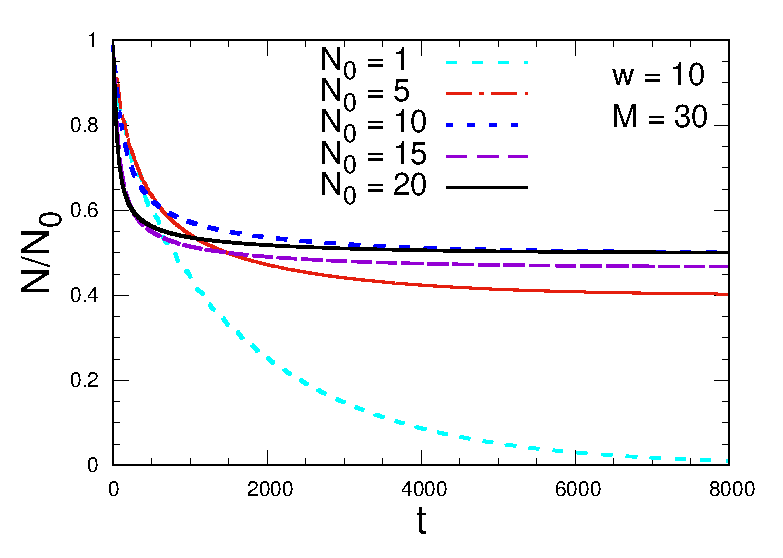
\includegraphics[width=0.65\columnwidth]{imm/Now10.eps}
    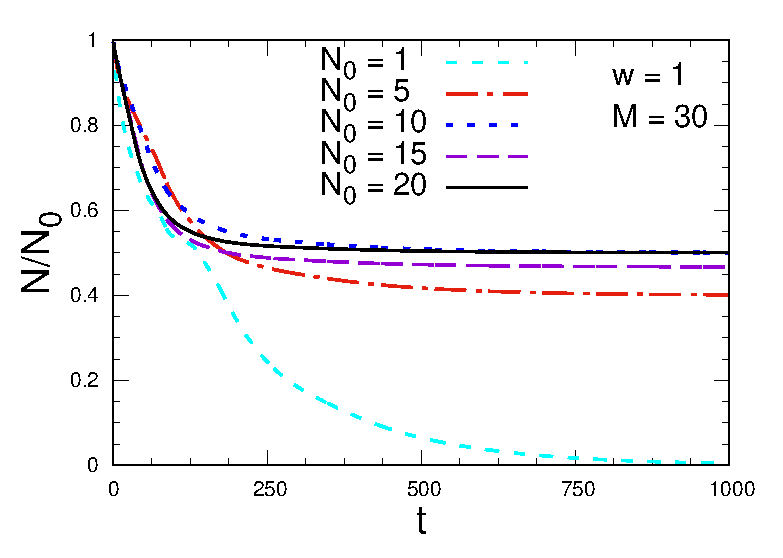
\includegraphics[width=0.65\columnwidth]{imm/No.eps}
    \caption{Behavior of the ratio $N(t)/N_0$ for the central-site
      particle-loss dissipation in systems of size $L=61$ ($M=30$)
      within hard walls, various initial particle number $N_0$, and
      dissipation localized at the center of the system, with $w=1$
      (bottom) and $w=10$ (top).  In both cases asymptotic stationary
      limit turns out to converge to $N/N_0=1/2$ for even $N_0$, and
      $N/N_0=(N_0-1)/(2N_0)$ for odd $N_0$.  Note that approach to the
      asymptotic value is slower for $w=10$ than $w=1$.}
    \label{ndiffn0}
  \end{figure}
  
  
  
  If we consider a central-site dissipation, thus $z=M+1=(L+1)/2$ [we
    recall that we are using shifted coordinates with respect to
    Eq.~(\ref{Hfree})], then the condition (\ref{kz}) reduces to $k=2j$,
  thus implying that $n_k$ remains unchanged for all even $k$ (whose
  odd-parity modes vanish at the central dissipative site), while it
  gets suppressed for odd $k$. Therefore, Eq.~(\ref{ddtnk}) implies that
  half of the fermions survives centrally localized decay
  dissipation. More precisely the stationary states are characterized by
  a residual particle number $N_{\rm asy} = N_0/2$ for even $N_0$, and
  $N_{\rm asy} = (N_0-1)/2$ for odd $N_0$.
  
  Note that the particle loss localized at the center, preserving the
  parity symmetry with respect to the center of the chain, is the
  optimal one to keep a fraction of fermionic particles at large time.
  For example, in the case of a dissipation at the boundaries, i.e.,
  when $z=1$ or $z=M$ in Eq.~(\ref{ddtnk}), no particles survive because
  all $k$-modes are involved by the Lindblad operator, leading to the
  complete suppression of the particles filling the initial ground
  state.
  
  \begin{figure}[!htb]
\centering
    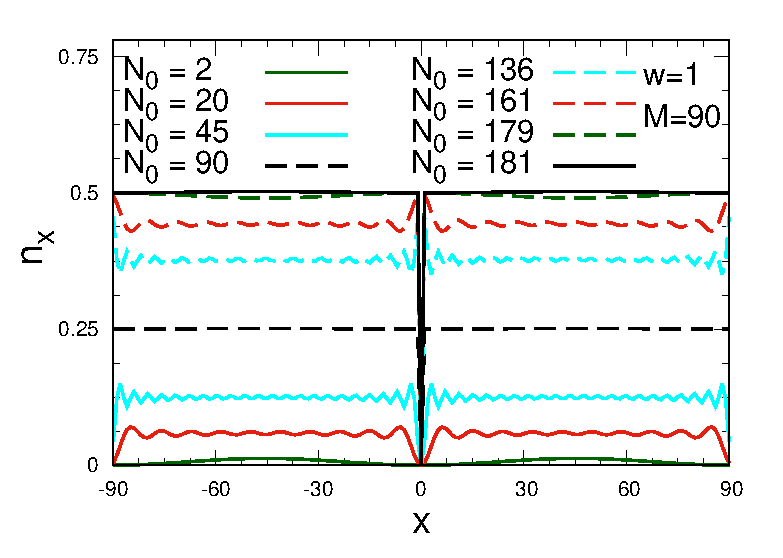
\includegraphics[width=0.65\columnwidth]{imm/nxhwall.eps}
    \caption{Data for the quantum evolution of the fermionic gas within
      hard walls, size $L=2M+1$ with $M=90$, initial particle number
      $N_0=10$, dissipation localized at the center of the chain with
      $w=1$. We show the particle density $n_x(t)$ at the sites $x=0$
      and $x=10$ (top), and the ratio $N(t)/N_0$ (bottom).  They
      approach asymptotic stationary limits (at least within the
      numerical precision, which is very accurate).}
    \label{nxdiffn0time}
  \end{figure}

  
  \begin{figure}[!htb]
\centering
    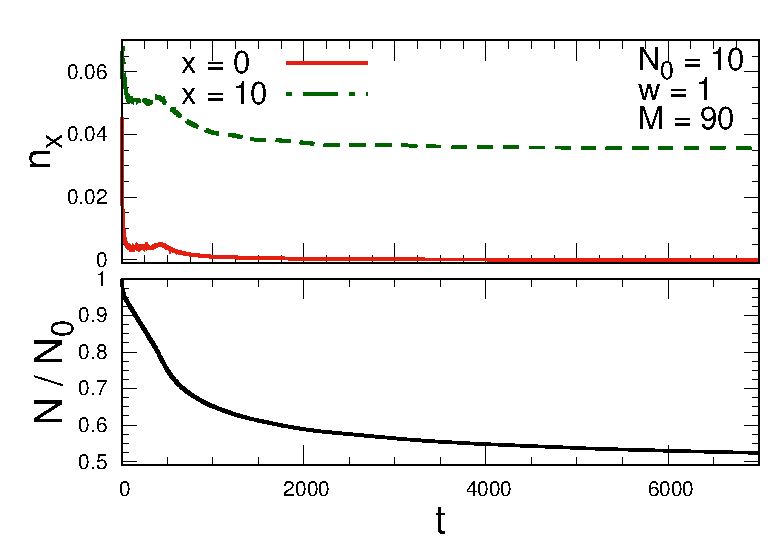
\includegraphics[width=0.65\columnwidth]{imm/nxNo.eps}
    \caption{Asymptotic stationary limit of the particle density $n_x$
      for systems of size $L=181$ ($M=90$) within hard-wall boundary
      conditions, in the presence of a central-site dissipation with
      $w=1$, and for various $N_0$. In all cases the particle density
      vanishes for $x=0$, and it is almost flat elsewhere, apart from
      small spatial oscillations, which appear similar to the
        Friedel oscillations characterizing the behavior of closed
        particle systems}.
    \label{nxdiffn0}
  \end{figure}
  
  
  The above analytical results are confirmed by the numerical results
  for the central particle-loss dissipation, see for example
  Fig.~\ref{ndiffn0} where we show the time dependence of the ratio
  $N(t)/N_0$ for various values of $N_0$ and $w$, and in particular the
  approach to its nonzero asymptotic limit. Also the space dependence of
  the particle density $n_x$ turns out to become stable asymptotically,
  approaching a stationary configuration, as shown in
  Fig.~\ref{nxdiffn0time}.  In Fig.~\ref{nxdiffn0} we show some results
  for the spatial dependence of the average particle density $n_x$ of
  the asymptotic stationary states. We note that $n_x$ is quite flat
  except at $x=0$ where the dissipative mechanism acts, and at the
  boundaries of the chain (essentially due to the hard-wall boundary
  conditions). The almost flat region shows some spatial oscillations,
  which appear suppressed when $N_0\approx M$ and $N_0\approx 2M$.
  
  
  \subsection{Approach to the asymptotic states}
  \label{asyappro}
  
  
  \subsubsection{Large-size behavior of the Liouvillian gap}
  \label{liogap}
  
  
  
  The approach to the stationary state is controlled by the Liouvillian
  gap $\Delta_{\cal L}$ of the generator ${\cal L}$ of the Lindblad
  equation~\cite{BP-openquantumsystembook,RH-book,Z-2015-relaxtimes,MBBC-18,KS-2020-boundarydephasing},
  \begin{equation}
  \Delta_{\cal L} = - {\rm Max}_{i>0} \, {\rm Re}\,(\Lambda_i)\,,
  \label{deltadeb}
  \end{equation}
  where $\Lambda_i$ are the eigenvalues of ${\cal L}$ (we recall that
  the largest eigenvalue is $\Lambda_0=0$ and ${\rm Re} \,\Lambda_i<0$
  for any $i>0$).  The Liouvillian gap for homogeneous spin chains and
  fermionic wires with localized dissipative mechanisms, such as that
  described by Eq.~(\ref{Lindop}), shows generally the asymptotic
  finite-size
  behavior~\cite{PP-08,P-2008-thirdquantization,Z-2015-relaxtimes,KS-2020-boundarydephasing,TV-2021-dissipativeboundaries}
  \begin{equation}
  \Delta_{\cal L}(w,L)\approx D_{\cal L}(w) \,L^{-3}\,.  
  \label{deltaL}
  \end{equation}
  We expect that this asymptotic large-$L$ behavior holds independently
  of the location of the particle-decay dissipation, and it does not
  depend on the initial conditions, thus on $N_0$.  The scaling equation
  (\ref{deltaL}) implies that the approach to the asymptotic behavior
  becomes slower and slower with increasing the size $L$ of the lattice
  at fixed $w$.
  
  \begin{figure}[!htb]
\centering
    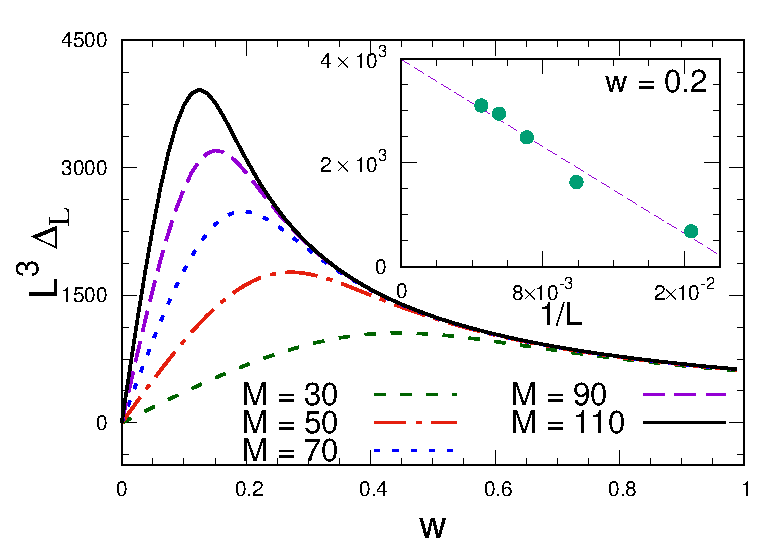
\includegraphics[width=0.65\columnwidth]{imm/DeltawNoL3.eps}
    \caption{The Liouvillian gap $\Delta_{\cal L}$ for particle-decay
      dissipation localized at the center of the chain, for various
      system size $L=2M+1$. The curves appear to converge with
      increasing $M$; this is clearly shown at least for $w\gtrsim 0.2$,
      as also shown by the large-$L$ convergence at a fixed value
      $w=0.2$ [suggesting that the corrections to the asymptotic scaling
      behavior (\ref{deltaL}) are approximately $O(L^{-1})$].  Like the
      case of dissipation at the boundaries, we believe that the
      convergence extends to any $w>0$, but, unlike dissipation at the
      boundaries, it is nonuniform when decreasing $w$ toward zero, see
      text.} 
    \label{liogaps}
  \end{figure}
  
  
  \begin{figure}[!htb]
\centering
    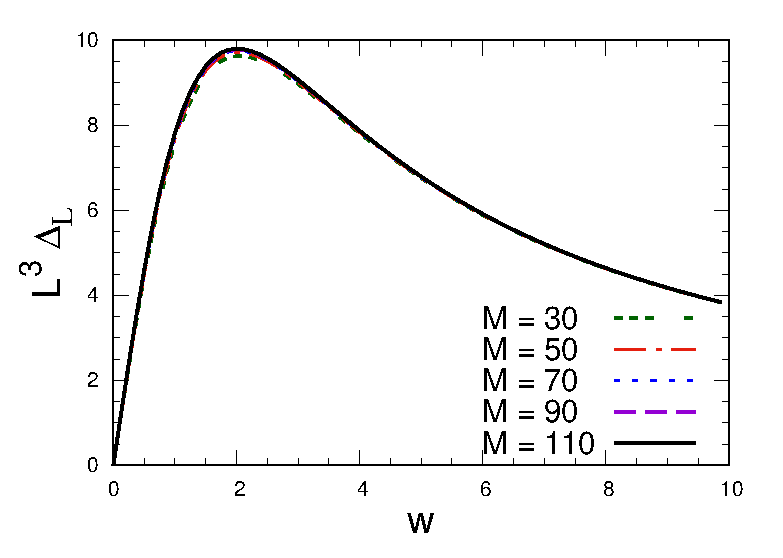
\includegraphics[width=0.65\columnwidth]{imm/deltaextr.eps}
    \caption{Scaling behavior of the Liouvillian gap $\Delta_{\cal L}$
      for particle-decay dissipation localized at one of the boundaries
      of the chain.}
        \label{liogapsb}
  \end{figure}
  
  
  
  
  \begin{figure}[!htb]
\centering
      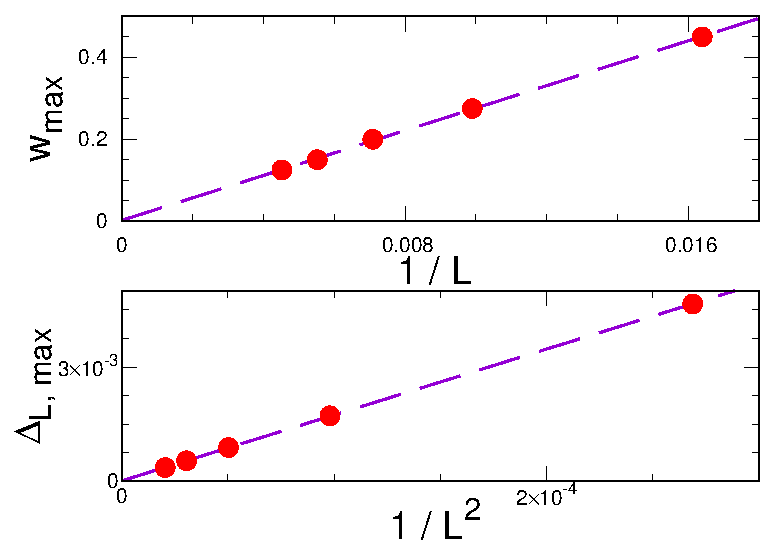
\includegraphics[width=0.65\columnwidth]{imm/wDmax1.eps}
    \caption{Some details of the behavior of the Liouvillian gap
      $\Delta_{\cal L}$ for dissipation localized at the center of the
      lattice. We show the location $w_{\rm max}$ of the maximum of the
      Liouvillian gap (top), showing that $w_{\rm max}\sim L^{-1}$, and
      value of $\Delta_{\cal L}$ at the maximum (bottom), showing that
      $\Delta_{\cal L}(w_{\rm max})\sim L^{-2}$.}
    \label{gapcenterdetails}
  \end{figure}
  
  
  \begin{figure}[!htb]
\centering
    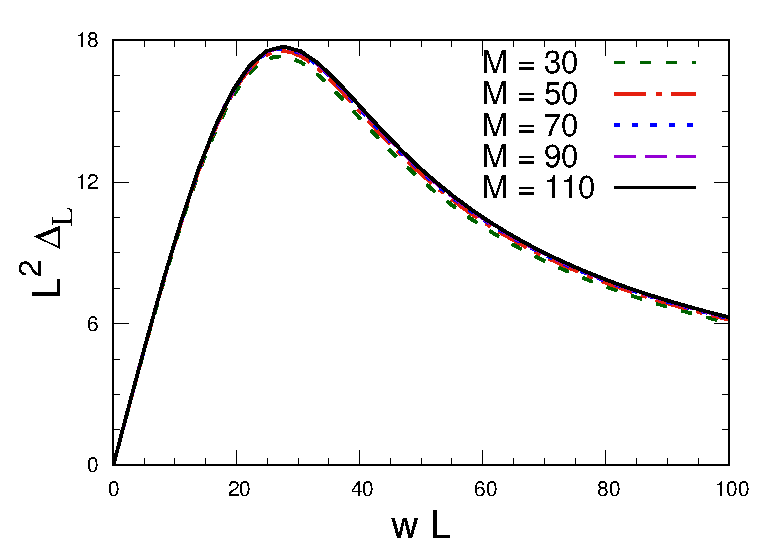
\includegraphics[width=0.65\columnwidth]{imm/DeltawLNo.eps}
    \caption{Plots of $L^2 \Delta_{\cal L}$ versus $wL$ for systems
      within hard walls and with central particle-loss dissipation, for
      various $L=2M+1$.  They support the scaling equation
      (\ref{deltaLcenter}).}
        \label{gapcenter2}
  \end{figure}
  
  The asymptotic behavior (\ref{deltaL}) is confirmed by numerical
  analyses of the Liouvillian gap using the method outlined in
  Ref.~\cite{PP-08}, see App.~\ref{appa}. Some numerical results are
  shown by Figs.~\ref{liogaps} and \ref{liogapsb}, for particle-decay
  dissipation localized at the center and at the boundary of the chain,
  respectively.
  
  In both cases, $\Delta_{\cal L}$ appears nonmonotonic, increasing for
  small values of $w$ and decreasing for sufficiently large dissipation
  strength $w$, for any $L$.  The approach to the asymptotic behavior
  becomes slower and slower with increasing $w$ for large $w$. In
  particular, $\Delta_{\cal L}(w,L)$ shows the large-$w$ behavior $L^3
  \Delta_{\cal L}(w)\approx D_{\cal L}(w)\sim w^{-1}$. This explains the
  results shown in Fig.~\ref{ndiffn0}, where the approach to the
  asymptotic value of the particle number for $w=10$ turns out to be
  slower than that for $w=1$.  The suppression in the limit of
    strong dissipation, for large $w$, may be interpreted as a
    quantum-Zeno-like phenomenon~\cite{MS-1977-quantumzeno,FP-08}, where a strong
    dissipation somehow slows down the dynamics, see
    e.g. Refs.~\cite{TNDTT-17,DMSD-20} for the appearence of similar
    quantum Zeno regimes.
  
  As shown by Figs.~\ref{liogaps} and \ref{liogapsb}, the Liouvillian
  gap at fixed $L$ has a maximum at an intermediate value of
  $w$. The corresponding values $w_{\rm max}$ and $L^3 \Delta_{\cal
      L}(w_{\rm max})$ appears to rapidly converge to the large-$L$
    limit in the case of dissipations localized at the boundaries, but
    they show an apparent size dependence in the case of dissipation
    localized at the center. Indeed the approach to the asymptotic
    $L^{-3}$ behavior (\ref{deltaL}) appears significantly slower in the
    case of dissipation localized at the center, in particular for small
    $w$, which suggests a nonuniform convergence for $w\to 0$.  The
    curves for different lattice sizes appear to clearly converge for
    $w\gtrsim 0.2$, as also shown by the inset of Fig.~\ref{liogaps}. We
    conjecture that, like the case of dissipation at the boundaries, the
    convergence in the large-size limit extends to any $w>0$, but it is
    nonuniform when decreasing $w$ toward zero, unlike dissipation at
    the boundaries.  This is demonstrated by the plots reported in
  Figs.~\ref{gapcenterdetails}, which show that the location of the
  maximum value of the Liouvillian gap for central dissipation moves
  toward $w=0$, with $w_{\rm max}\sim L^{-1}$, and its maximum value
  decreases as $\Delta_{\cal L}(w_{\rm max})\sim w_{\rm max}^2\sim
  L^{-2}$, instead of the general asymptotic $L^{-3}$ behavior for $w>0$
  fixed. Actually, they suggest that the Liovillian gap for central
  dissipation shows also the asymptotic scaling behavior
  \begin{equation}    
  \Delta_{\cal L}(w,L)\approx {\cal D}_{\cal L}(wL) \,L^{-2}\,,
  \label{deltaLcenter}
  \end{equation}
  obtained in the large-$L$ limit keeping $wL$ constant.  This scaling
  behavior is demonstrated by the plot reported in
  Fig.~\ref{gapcenter2}.  Therefore the function $D_{\cal L}(w)$
  entering the asymptotic $L^{-3}$ behavior (\ref{deltaL}) must be
  singular for $w\to 0$ in the case of central-site dissipation,
  diverging as $w^{-1}$.
  
  Note that the above considerations on the behavior of the Liouvillian
  gap apply to generic values of $w$, and,  of course, they do not depend
  on the initial number $N_0$ of particles.  In the following we will
  mainly present results for the value $w=1$ of the dissipation
  parameter, whose dynamic scenarios are shared with those arising from
  generic finite values of $w$.
  
  \subsubsection{Large-time behavior of the particle number}
  \label{lasypgap}
  
  On the basis of the large-size behavior of the Liouvillian gap, we
  expect that the time scale $t_a$ of the approach to the stationary
  state is given as
  \begin{equation}
  t_a \sim \Delta_{\cal L}^{-1}\sim L^3\,,
  \label{timescaleasy}
  \end{equation}
  at fixed $w>0$. This time scale must characterize the approach to the
  stationary limits of the particle number and density.  This is
  confirmed by the numerical computations, see for example
  Fig.~\ref{rntn010} where we report results for the ratio
  \begin{equation}
    R_N(t)\equiv {N(t)-N_{\rm asy}\over N_0-N_{\rm asy}}\,,
      \label{defqu}
  \end{equation}
  for protocols starting from a fixed number $N_0$ of particles.  They
  show the asymptotic large-$L$ scaling behavior
  \begin{eqnarray}
    R_N(t,w,L) \approx A(t/L^3,w)\,,\label{scalbehasy}
  \end{eqnarray}
  which also implies
  \begin{eqnarray}
  {d R_N(t,w,L)\over dt} &\approx& L^{-3} B(t/L^3,w)\,.  \nonumber
  \end{eqnarray}
  Analogous results are obtained for the case we start from a fixed
  ratio $N_0/M$, as shown in Fig.~\ref{dntln0lasy} for $N_0/M=1/2$,
  where we plot $N(t)-N_{\rm asy}$ versus $t/L^3$ and the curves appear
  to collapse in the large-$M$ limit. Note that when $N_0/M$ is kept
  fixed, the quantity $R_N$ defined in Eq.~(\ref{defqu}) is not
  appropriate, because it is always suppressed in the large-time limit,
  due to the denominator that behaves as $N_0-N_{\rm asy}\sim L$.
  
  
  \begin{figure}[!htb]
\centering
    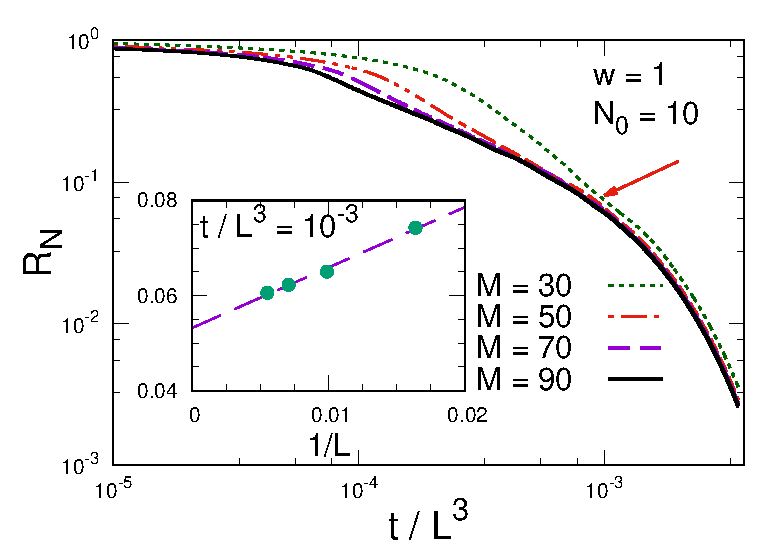
\includegraphics[width=0.65\columnwidth]{imm/NL3.eps}
    \caption{The time dependence of the ratio $R_N$ versus $t/L^3$
      ($L=2M+1$), for homogenous systems within hard walls with $N_0=10$
      and central particle-loss dissipation with $w=1$.  The data for
      various sizes $M$ show clearly the convergence toward a dynamic
      scaling curve, approximately as $1/L$ as shown by the inset for a
      particular value of the ratio $t/L^3$ (the one indicated by the
      arrow in the main figure).}
    \label{rntn010}
  \end{figure}
  
  
  \begin{figure}[!htb]
\centering
    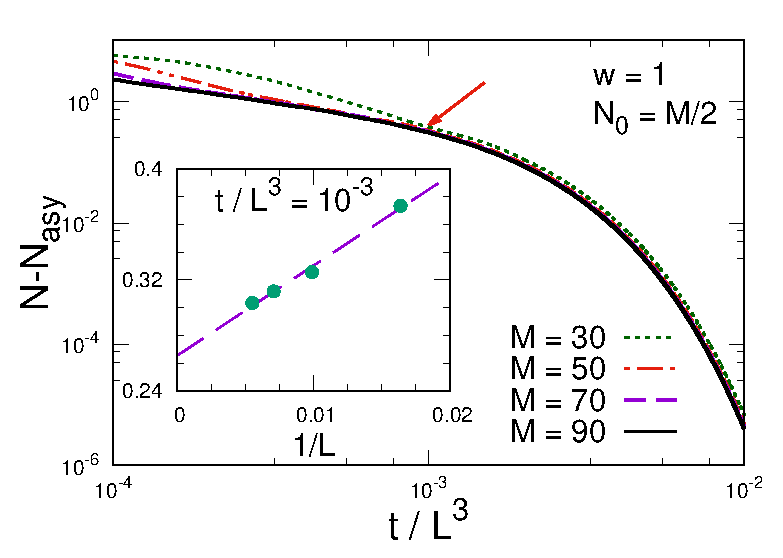
\includegraphics[width=0.65\columnwidth]{imm/dNLL3.eps}
    \caption{The difference $N(t) - N_{\rm asy}$ vs $t/L^3$, for systems
      within hard walls with $N_0/M=1/2$, and central dissipation with
      $w=1$.  Again we observe the asymptotic convergence toward a
      dynamic scaling curve, as shown by the inset for a particular
      value of $t/L^3$ (indicated by the arrow in the main figure).}
    \label{dntln0lasy}
  \end{figure}
  
  As we will show below, this is not the end of the story, indeed
  further peculiar intermediate scaling behaviors emerge, differing
  between the cases $N_0$ and $N_0/M$ fixed.
  
  
  
  
  \subsection{Intermediate scaling behaviors keeping $N_0$ fixed}
  \label{N0fixed}
  
  \begin{figure}[!htb]
\centering
    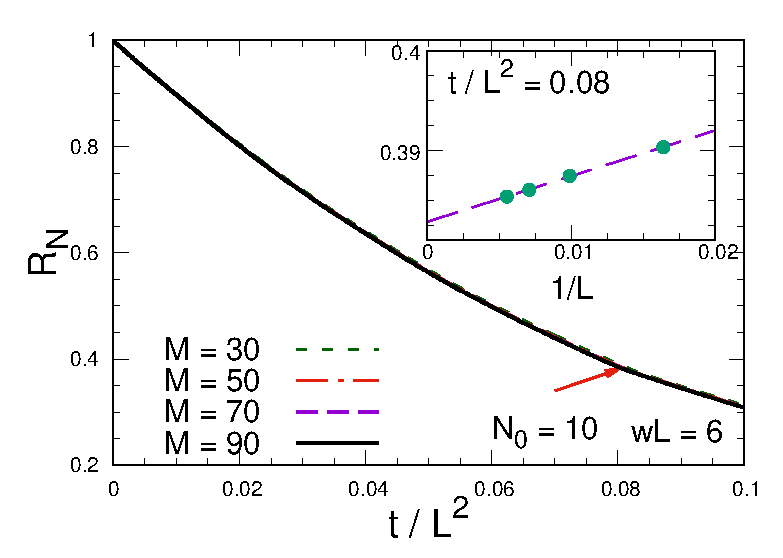
\includegraphics[width=0.65\columnwidth]{imm/NwL2.eps}
    \caption{The ratio $R_N$ versus $t/L^2$ for systems within hard
      walls with $N_0=10$, central dissipation with $wL=6$, for various
      lattice sizes $L=2M+1$.  The data appear to converge toward a
      scaling curve in the large-$L$ limit, as demonstrated by the data
      reported in the inset for a particular value of the ratio
      $t/L^2$.}
    \label{rntn010ir}
  \end{figure}
  
  We now look for intermediate regimes of the time evolution, somehow
  associated with the time scales of the Hamiltonian (\ref{Hfree})
  driving the unitary dynamics, and therefore to its gap $\Delta_H$,
  i.e. the energy difference between the first excited state and the
  ground state. When keeping the particle number $N_0$ fixed, $\Delta_H$
  behaves asymptotically as $\Delta_H \sim L^{-2}$, corresponding to the
  dynamic exponent $z=2$ of the vacuum-superfluid
  transition~\cite{S99}.
  
  We want to check whether the
    out-of-equilibrium dynamics develops an intermediate regimes somehow
    controlled by the Hamiltonian driving of the Lindblad equation,
    whose intrinsic time scale is related to its gap, i.e. $t \sim
    \Delta_H^{-1}\sim L^2$, which is much smaller than the time scale
    $t\sim L^3$ characterizing the approach to the stationary large-time
    limit (of course, for sufficiently large $L$, and in particular in
    the large-$L$ limit). As we shall see, a closer look at the time
    evolution provides a clear evidence of such intermediate regime, which 
     also requires a rescaling of the dissipation strength.
  
  
  In Fig.~\ref{rntn010ir} we show some results for the time dependence
  of the particle number in the case of systems with central-site
  dissipation starting from a fixed number of particles. We observe that
  the above-mentioned intermediate regime exists, and extends to any
  $t\sim L^2$, if we perform an appropriate rescaling of the dissipation
  parameter $w$, decreasing $w$ as $w\sim L^{-1}$. Indeed the numerical
  results clearly support the large-$L$ scaling behavior
  \begin{eqnarray}
   R_N(t,w,L) \approx U(t/L^2,wL)\,,   \label{scalbehwl}
  %%  L^2 {d R_N(t,w,N_0,L)\over dt} &\approx& W(t/L^2,wL)\,,\nonumber
  \end{eqnarray}
  which is obtained by increasing $L$ keeping the ratio $t/L^2$ and the
  product $wL$ fixed.  Note that this intermediate scaling behavior is
  expected to hold even for large values of the ratio $t/L^2$, because
  it is also compatible with the alternative scaling behavior
  (\ref{deltaLcenter}) of the Liouvillian gap.
  
  
  
  
  
  
  \subsection{Intermediate dynamic behavior keeping $N_0/M$ fixed}
  \label{N0oLfixed}
  
  \begin{figure}[!htb]
\centering
    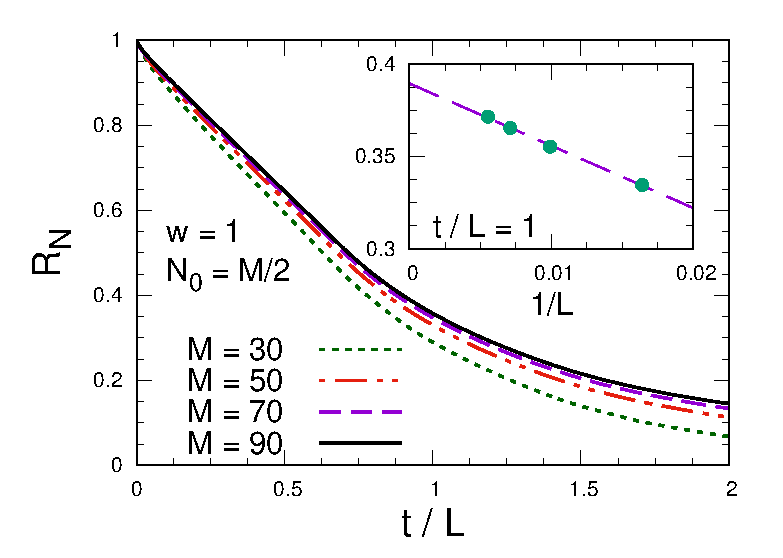
\includegraphics[width=0.65\columnwidth]{imm/NLL1.eps}
    \caption{Behavior of the ratio $R_N$ versus $t/L$, for systems
      within hard walls with $N_0/M=1/2$, and central dissipation with
      $w=1$. The inset shows the $1/L$ approach to the large-$L$
      asymptotic behavior.}
    \label{rntn0lvstol}
  \end{figure}
  
  We now consider the large-$L$ behavior in the case we keep the ratio
  $N_0/M$ fixed when increasing $L=2M+1$. This corresponds to the
  superfluid phase, i.e. when the chemical potential $\mu$ is larger
  than that at the vacuum-superfluid transition, $\mu>-2$. Within the
  superfluid phase, the gap $\Delta_S$ of isolated free Fermi gases
  behaves as~\cite{S99} $\Delta_S \sim L^{-1}$.
  
  Again we want to check whether the out-of-equilibrium dynamics in
    this condition develops an intermediate regime controlled by the
    part of the Lindblad equation driving the unitary dynamics
    introduces a time scale $t\sim \Delta_S^{-1}\sim L$ (again, much
    smaller than the time scale $t\sim L^3$ characterizing the approach
    to the stationary large-time limit). Like the case at fixed $N_0$,
    we show that such an intermediate regime exists.
  
  The existence of a corresponding intermediate regime of the dynamics
  is demonstrated by the results shown in Fig.~\ref{rntn0lvstol},
  leading to the intermediate scaling ansatz
  \begin{eqnarray}
   R_N(t,w,L) \approx W(t/L,w)\,,   \label{scalbehnol}
  %%  L {d R_N(t,w,L)\over dt} &\approx& W(t/L,w)\,,\nonumber
  \end{eqnarray}
  obtained keeping $t/L$ fixed in the large-$L$ limit.  
  
  We finally report the existence of a further early-time regime when we
  start from the ground state for $N_0\propto M$, as already noted in
  Ref.~\cite{FMKCD-20}. Indeed, for sufficiently small time
  \begin{equation}
    {d N(t,w,L)\over dt} \approx  f(t,w)\,,
    \label{vereg}
    \end{equation}
  without showing any asymptotic size dependence.  This is shown by the
  curves reported in Fig.~\ref{rntln0lvst}.  The behavior (\ref{vereg})
  is observed in the large-size limit, and can be considered as the {\em
    thermodynamic} limit of the quantum evolution, when the time is
  sufficiently small that the dynamics does not yet detect the effects
  of the boundaries.  Indeed deviations are observed for $t\propto M$,
  thus later and later for larger and larger systems. At the end of this
  early-time regime, the intermediate regime (\ref{scalbehnol}) begins.
  
  
  
  \begin{figure}[!htb]
\centering
  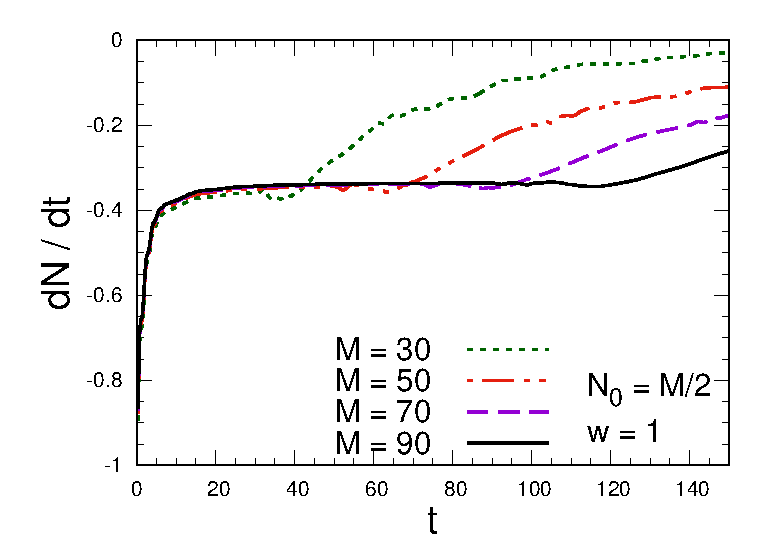
\includegraphics[width=0.65\columnwidth]{imm/dNLL0.eps}
  \caption{The time dependence of the derivative of the particle number,
    for systems within hard walls with central-site dissipation with
    $w=1$, starting from ground states with $N_0/M=1/2$ fixed.  }
    \label{rntln0lvst}
  \end{figure}
  
  
  
  \section{Fermionic gases within harmonic traps}
  \label{hartra}
  
  
  We now present results for lattice fermionic systems within traps
  arising from inhomogeneous external potentials, such as those in
  Eq.~(\ref{potential}), in the presence of a particle-decay dissipation
  at the center of the trap, as described by the Lindblad equations
  (\ref{EQLindblad}) and (\ref{Lindop}). As already mentioned in
    the introductive section, effective harmonic trapping mechanisms are
    quite common in cold-atom experiments~\cite{BDZ-08}. Therefore their
    analysis is also relevant from a phenomonological point of view.
  
  We study the time evolution in the limit of large trap size $L_t$, in
  the case we keep the initial particle number $N_0$ fixed, and when we
  keep the ratio $N_0/L_t$ constant (equivalent to addiing a chemical
  potential). We consider harmonic traps, thus $p=2$ in
  Eq.~(\ref{potential}). The results are obtained for sufficiently large
  systems $L$ at fixed $L_t$, so that a further increases of $L$ does
  not change the results at fixed $L_t$, and therefore they can be
  considered as results for infinite-size systems with a large accuracy,
  within the accuracy of the numerical calculations, better than
  $10^{-8}$.
  
  
  \subsection{Large-time behavior}
  \label{asytrap}
  
  \begin{figure}[!htb]
\centering
    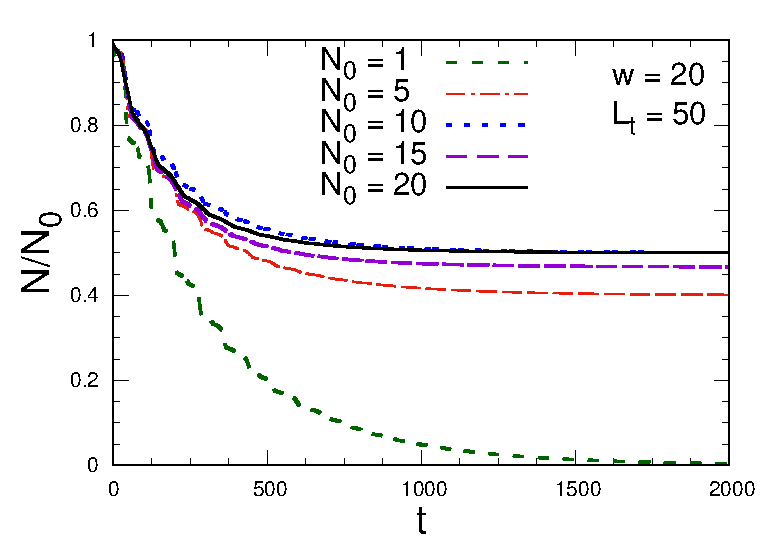
\includegraphics[width=0.65\columnwidth]{imm/trapNow20.eps}
  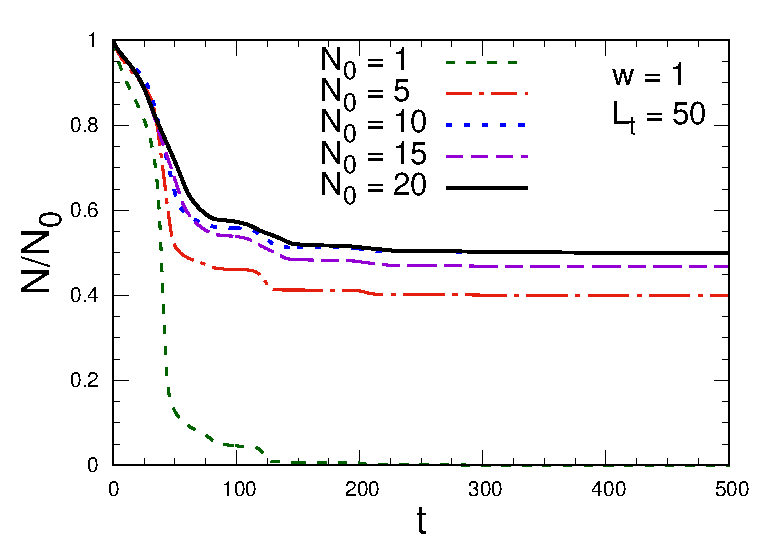
\includegraphics[width=0.65\columnwidth]{imm/trapNo.eps}
  \caption{The time dependence of the ratio $N/N_0$ for the central-site
    particle-loss dissipation $w=1$ (bottom) and $w=20$ (top) in systems
    within harmonic traps, various $N_0$, and $L_t=50$ (in the large-$L$
    limit to make the finite-size effects negligible).  The asymptotic
    stationary limit turns out to converge to $N/N_0=1/2$ for even
    $N_0$, and $N/N_0=(N_0-1)/(2N_0)$ for odd $N_0$. Similarly to the
    case of systems within hard walls, see Fig.~\ref{ndiffn0}, the
    approach to the asymptotic value turns out to be slower for $w=20$
    than $w=1$.}
  \label{traptdep}
  \end{figure}
  
  
  To begin with, we discuss the asymptotic stationary states.  In
  Fig.~\ref{traptdep} we show the time dependence, and asymptotic
  behavior, of the ratio $N(t)/N_0$ for various values of the initial
  number of particles. Again, similarly to the case of homogeneous
  systems within hard walls and particle-decay dissipation at the center
  of the chain, we find that the large-time states keep a half of the
  initial particles.  Analogously to the hard-wall case, this can be
  related to the fact that the one-particle Hamiltonian is invariant
  under reflections with respect to the center, thus the one-particle
  states must have definite parity. This can be easily seen in the
  continuum limit, see e.g. Ref.~\cite{ACV-14}, where the one-particle
  Hamiltonian eigenfunctions can be written in terms of Hermite
  polynomials, and have definite parity.  Since the one-particle states
  with negative parity vanishes at the center of the trap, the
  corresponding modes in the ground state of the fermionic system are
  not affected by the particle-decay dissipation at the center of the
  trap. Then, recalling that the ground state is obtained by filling the
  first $N_0$ one-particle levels, a selection mechanism analogous to
  that identified in the case of homogeneous systems applies, see
  Sec.~\ref{asysta}, therefore half of them are odd [more precisely
    $N_0/2$ for even $N_0$ and $(N_0-1)/2$ for odd $N_0$], we expect
  again that half particles survive the central particle loss.
  
  \begin{figure}[!htb]
\centering
  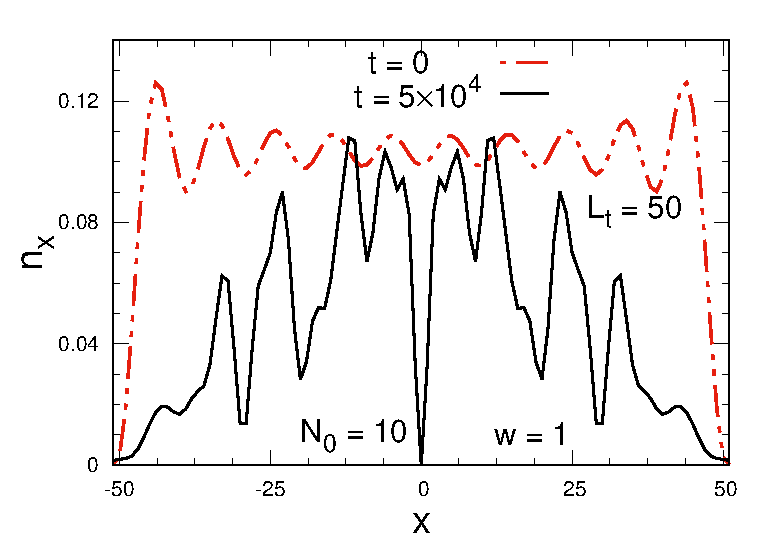
\includegraphics[width=0.65\columnwidth]{imm/trapnxLt50.eps}
  \caption{The particle density $n_x$ for systems within a harmonic trap
    with initial particle number $N_0=10$, at $t=0$ and after some time
    $t$, for a central dissipation with $w=1$, fixed trap size $L_t=50$,
    and for a sufficiently large size of the system, $L=221$, to make
    finite-size effects negligible (numerically checked by verifying the
    dependence on $L$).}
  \label{trapnxt}
  \end{figure}
  
  In Fig.~\ref{trapnxt} we show the particle density at $t=0$ and at
  large time when the central particle density has already stably
  vanished. However, the spatial dependence of the particle density does
  not appear static in the large-time regime where the particle number
  stops decreasing. Indeed, as shown in Fig.~\ref{trapnxto}, the time
  dependence of the particle density at sites $x\neq 0$ is characterized
  by time oscillations that apparently continue indefinitely, persisting
  even in the large-$L_t$ limit.  We also note that in this large-time
  regime the quantum evolution of the particle density appears
  effectively driven by the Hamiltonian term only. We have checked that
  the dissipative contribution in Eq.~(\ref{eqscxytrap}), i.e. the one
  proportional to $w$, gets suppressed asymptotically, thus only the
  Hamiltonian determines the large-time dependence of the fixed-time
  two-point function ${\mathscr C}_{xy}(t)$ and $n_x={\mathscr
    C}_{xx}(t)$. In this large-time regime also the energy of the system
  defined in Eq.~(\ref{enedef}) remains constant, indeed its time
  derivative vanishes when ${\rm Re}\,{\mathscr C}_{0,1}=0$,
  cf. Eq.~(\ref{derene}).
  
  
  
  
  
  
  \begin{figure}[!htb]
\centering
  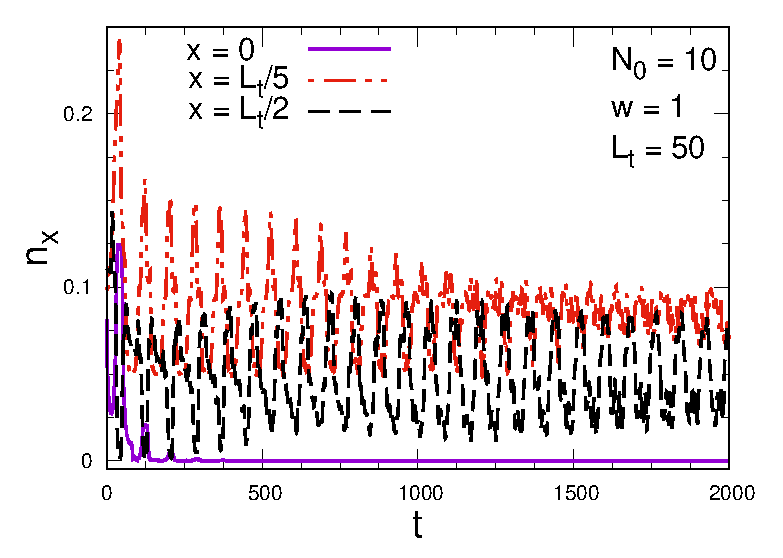
\includegraphics[width=0.65\columnwidth]{imm/nxtLt50.eps}
  \caption{ Time dependence of the particle density for systems within a
    trap of size $L_t=50$, at various spatial coordinates, $x=0$,
    $x=L_t/5=10$ and $x=L_t/2=25$, for central dissipation with $w=1$.
    The particle density $n_x$ for $x\neq 0$ are characterized by
    oscillations in the large-time regime, when $n_x$ at $x=0$ and the
    particle number have already approached their asymptotic behavior.
  }
  \label{trapnxto}
  \end{figure}
  
  
  \subsection{Large-$L_t$ scaling behavior of the time dependence}
  \label{trapscaling}
  
  
  The time dependence starting from a fixed number of particles shows
  the peculiar scaling behavior
  \begin{equation}
    R_N(t,w,L_t) \equiv {N(t)-N_{\rm asy}\over N_0-N_{\rm asy}} \approx
    A_t(t/L_t,w)\,,
    \label{rntrapn0}
  \end{equation}
  which apparently describes the whole time evolution.  This is clearly
  supported by the data reported in Figs.~\ref{trapNo} and
  \ref{trapNow01} for central dissipation with $w=1$ and initial
  particle number $N_0=10$.
  
  Note that the time scale $t\sim L_t$ may be also related to the gap of
  the fermionic Hamiltonian, for which $\Delta_{L_t} \sim
  L_t^{-z\theta}$ where $z=2$ is the dynamic exponent associated with
  the vacuum-to-superfluid transition, and $\theta=1/2$ is the universal
  trap exponent characterizing critical behaviors in the presence of
  trapping potentials~\cite{CV-09,CV-10,ACV-14,rossini2021coherent} [for generic
    power laws of the potential (\ref{potential}), $\theta=p/(p+2)$].
  
  \begin{figure}[!htb]
\centering
  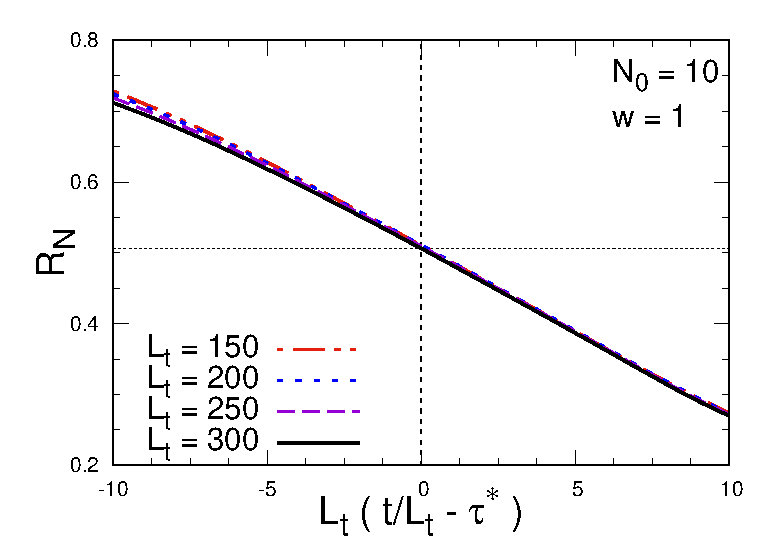
\includegraphics[width=0.65\columnwidth]{imm/crit.eps}
  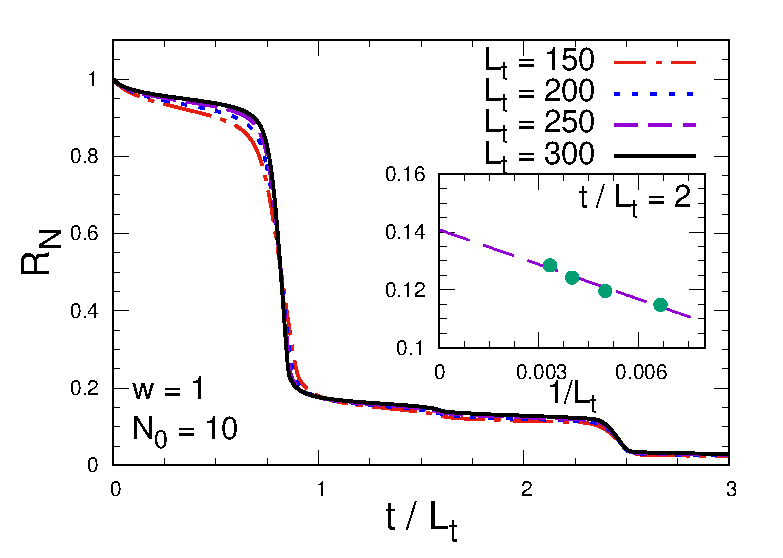
\includegraphics[width=0.65\columnwidth]{imm/RNtrapNo.eps}
  \caption{ The bottom figure shows the time evolution of the ratio
    $R_N$ versus $t/L_t$ for $w=1$, various trap sizes, keeping the
    initial number of particles $N_0=10$ fixed.  The inset shows an
    example of convergence at $t/L_t=2$.  The top figure shows the
    scaling behavior at the fast drop of the particle number, around
    $t/L_t\approx 0.8147$, described by Eq.~(\ref{atcrit}).  }
  \label{trapNo}
  \end{figure}
  
  \begin{figure}[!htb]
\centering
  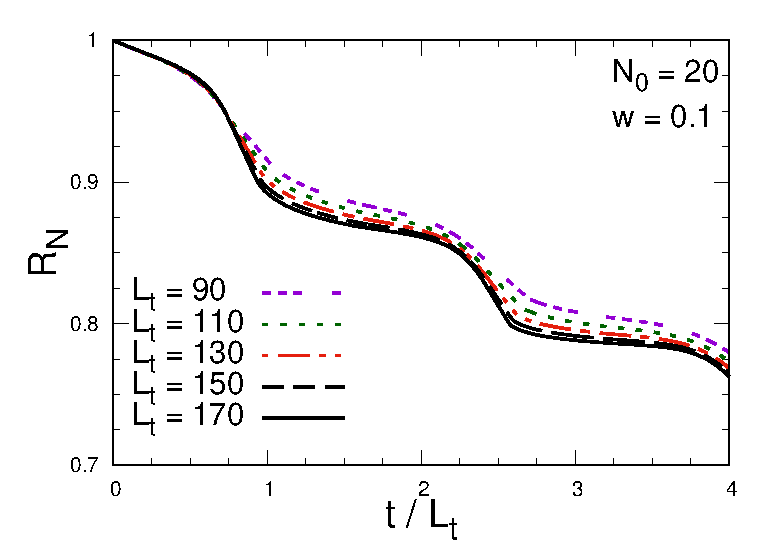
\includegraphics[width=0.65\columnwidth]{imm/RNtrapNo20w01.eps}
  \caption{The ratio $R_N$ for $w=0.1$, various trap sizes, keeping the
    initial number of particles $N_0=20$ fixed.}
  \label{trapNow01}
  \end{figure}
  
  \begin{figure}[!htb]
\centering
  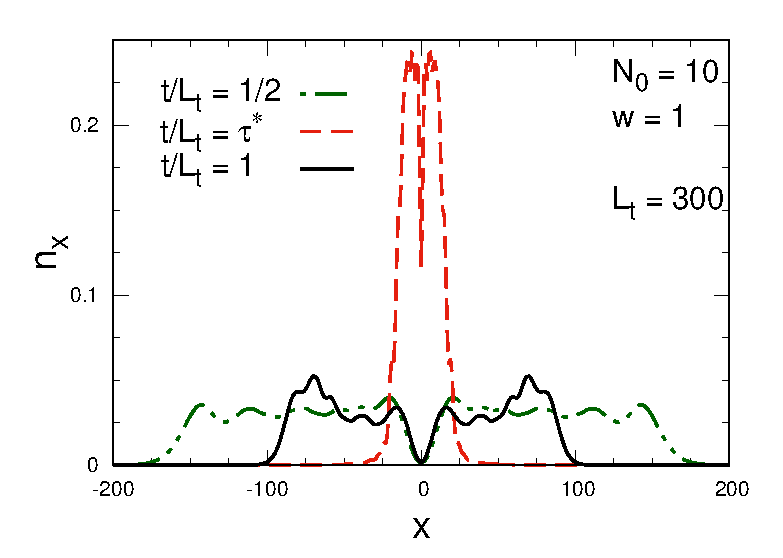
\includegraphics[width=0.65\columnwidth]{imm/nxtrap.eps}
  \caption{ Behavior of the particle density around the singularity of
    the scaling function (\ref{rntrapn0}), for $L_t=300$, central
    particle loss with $w=1$, and some values of the ratio $t/L_t$
    around the singular point $t/L_t =\tau^*\approx 0.8147$. They show
    that large drop of the particle number at $\tau^*$ is connected with
    a simultaneous large increase of the particle density at the center
    of the trap.  }
  \label{trapnx}
  \end{figure}
  
  
  
  
  
  The time scale $t\sim L_t$ characterizes the whole evolution of the
  system, up to the large-time regime, except for some small
  intermediate time intervals. Indeed, the curves shown in the bottom
  Fig.~\ref{trapNo} presents some flat regions followed by rapid
  changes.  Actually a more careful analysis, see, e.g., the top
  Fig.~\ref{trapNo}, shows that the scaling function $A_t(t/L_t,w)$
  entering Eq.~(\ref{rntrapn0}) appears to develop a singularity in the
  large-time limit, at $t/L_t = \tau^*\approx 0.8147$, so that
  \begin{equation}
    A_t(t/L_t,w) \approx f[L_t (t/L_t-\tau^*)]
    \label{atcrit}
  \end{equation}
  around $t/L_t=\tau^*$. Therefore this sharp drop of the particle
  density occurs at a time $t^* \approx L_t \tau^*$ in the large-$L_t$
  limit, and lasts for a finite time interval, i.e. it does not diverge
  when increasing $L_t$.  Some data for the behavior of the particle
  density and number around the time $\tau^*$ are shown in
  Fig.~\ref{trapnx}, where we note the significant increase of the
  particle density around $x=0$ when the singular behavior of the
  scaling function (\ref{rntrapn0}) appears.  Analogous behaviors are
  observed for generic values of $N_0$ and $w$.
  
  
  In the case we keep $N_0/L_t$ fixed, the results show a generic
  scaling behavior in terms of $t/L_t$, analogous to
  Eq.~(\ref{rntrapn0}), see for example Fig.~\ref{trapNoLt}.
  
  
  
  
  
  
  \begin{figure}[!htb]
\centering
  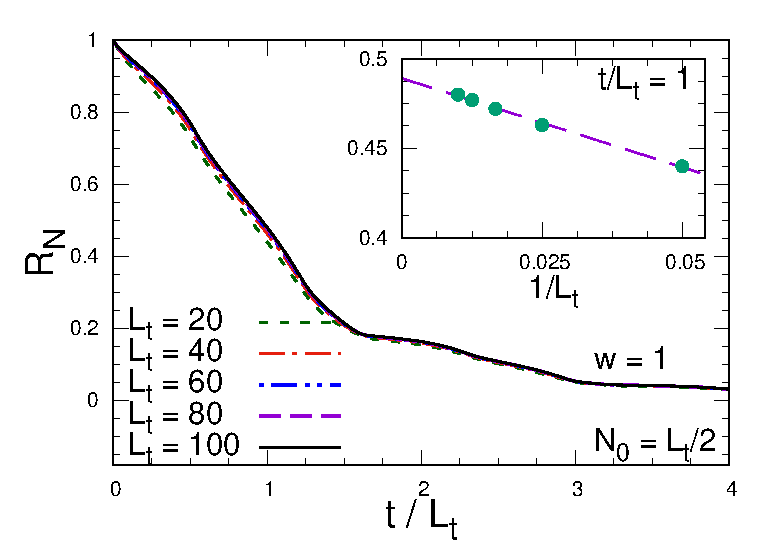
\includegraphics[width=0.65\columnwidth]{imm/RNtrapNoLt.eps}
  \caption{ Time evolution of the ratio $R_N$ versus $t/L_t$ for
    fermionic gases within harmonic traps of various size, keeping the
    ratio $N_0/L_t=1/2$ fixed, for central particle-loss dissipation with
    $w=1$. The  large-$L_t$ convergence is evident, as also shown by
    the plot reported within the inset. }
  \label{trapNoLt}
  \end{figure}
  